        %%******************************************%%
        %%                                          %%
        %%        Modello di tesi di laurea         %%
        %%            di Andrea Giraldin            %%
        %%                                          %%
        %%             2 novembre 2012              %%
        %%                                          %%
        %%******************************************%%

\begin{document}
    \frontmatter
    \begin{titlepage}
    \begin{center}
        \begin{LARGE}
            \textbf{\myUni}\\
        \end{LARGE}

        \vspace{10pt}

        \begin{Large}
            \textsc{\myDepartment}\\
        \end{Large}

        \vspace{10pt}

        \begin{large}
            \textsc{\myFaculty}\\
        \end{large}

        \vspace{30pt}
        \begin{figure}[htbp]
            \centering
            
\includegraphics[height=5cm]{unipd-logo.png}
        \end{figure}
        \vspace{30pt}

        \begin{LARGE}
            \textbf{\myTitle}\\
        \end{LARGE}

        \vspace{10pt}

        \begin{large}
            \textsl{\myDegree}\\
        \end{large}

        \vspace{40pt}

        \begin{large}
            \begin{flushleft}
                \textit{Supervisor}\\
                \vspace{5pt}
                \profTitle\ \myProf
            \end{flushleft}

            % You can tweak the spacing to have professor and student names on the same line
            % useful if the page is broken by a long thesis title and you need more space
            \vspace{-52pt}

            \begin{flushright}
                \textit{Candidate}\\
                \vspace{5pt}
                \myName \\
                \vspace{5pt}
                \textit{ID} \myID
            \end{flushright}
        \end{large}

        \vspace{40pt}

        \line(1, 0){338} \\
        \begin{normalsize}
            \textsc{Academic Year \myAA}
        \end{normalsize}
    \end{center}
\end{titlepage}

    \clearpage
\phantomsection
\thispagestyle{empty}

\hfill
\vfill

\noindent\myName: \textit{\myTitle,}
\myDegree,
\textcopyright\ \myTime.

    \cleardoublepage
\phantomsection
\thispagestyle{empty}
\pdfbookmark{Dedica}{Dedica}

\vspace*{3cm}

\begin{center}
    Lorem ipsum dolor sit amet, consectetuer adipiscing elit. \\ \medskip
    --- Oscar Wilde
\end{center}

\medskip

\begin{center}
    Dedicato a ...
\end{center}

    \cleardoublepage
\phantomsection
\pdfbookmark{Summary}{summary}
\begingroup
\let\clearpage\relax
\let\cleardoublepage\relax
\let\cleardoublepage\relax

\chapter*{Summary}

This document describes the work done during the 750-hours final project at \href{https://www.221e.com/about-us}{221e S.r.l.}\\
The project's goal is to architect and develop a cloud-based system capable of ingesting and processing data from heterogeneous IoT sensors so that a knowledge database can be built.\\
The system must be designed to be scalable and fault-tolerant, and it must be platform-agnostic.\\
This document is going to describe the company, the idea behind the project, the work done and an assessment of what I developed and learned during my internship.\\

%\vfill

%\selectlanguage{english}
%\pdfbookmark{Abstract}{Abstract}
%\chapter*{Abstract}

%\selectlanguage{italian}

\endgroup

\vfill

    \cleardoublepage
\phantomsection
\pdfbookmark{Acknowledgements}{acknowledgements}

\begin{flushright}{
    \slshape
    ``Te ghe da pomparghe drio''} \\
    \medskip
    --- Federico Gallo
\end{flushright}


\bigskip

\begingroup
\let\clearpage\relax
\let\cleardoublepage\relax
\let\cleardoublepage\relax

\chapter*{Acknowledgements}

\noindent \textit{Prof. \myProf, my thesis supervisor, deserves my deepest gratitude for his exceptional support and guidance throughout the completion of this research.}\\
\noindent \textit{My family, for their encouragement and understanding throughout this academic endeavour, has my heartfelt thanks.}\\
\noindent \textit{I am truly grateful to Luca Perosa, Bledar Gogaj, Marco Lionello, and all my peers at SCAI ITEC, for their unwavering support when I made the decision to pursue a Master’s degree.}\\
\noindent \textit{I extend my sincere appreciation to PhD. Roberto Bortoletto, my company tutor, and all my colleagues in 221e for their invaluable support and guidance throughout my final project.}\\
\noindent \textit{Last but not least, I want to give a shoutout to all my friends for having my back and just being there through high and lows. Your friendship means a lot to me, and I appreciate the support and good times we've shared.}\\
\bigskip

\noindent\textit{\myLocation, \myTime}
\hfill \myName

\endgroup

    \cleardoublepage
\pdfbookmark{\contentsname}{tableofcontents}
\setcounter{tocdepth}{2}
\tableofcontents
%\markboth{\contentsname}{\contentsname}
\clearpage

\begingroup
    \let\clearpage\relax
    \let\cleardoublepage\relax
    \let\cleardoublepage\relax

    % Figures list
    \phantomsection
    \pdfbookmark{\listfigurename}{lof}
    \listoffigures

    \vspace*{8ex}

    % Tables list
    \phantomsection
    \pdfbookmark{\listtablename}{lot}
    \listoftables

    \vspace*{8ex}
\endgroup

\cleardoublepage

    \cleardoublepage

    \mainmatter
    \chapter{Introduzione}
\label{cap:introduzione}

Introduzione al contesto applicativo.\\

\noindent Esempio di utilizzo di un termine nel glossario \\
\gls{api}. \\

\noindent Esempio di citazione in linea \\
\cite{site:agile-manifesto}. \\

\noindent Esempio di citazione nel pie' di pagina \\
citazione\footcite{womak:lean-thinking} \\

\section{L'azienda}

Descrizione dell'azienda.

\section{L'idea}

Introduzione all'idea dello stage.

\section{Organizzazione del testo}

\begin{description}
    \item[{\hyperref[cap:processi-metodologie]{Il secondo capitolo}}] descrive ...
    
    \item[{\hyperref[cap:descrizione-stage]{Il terzo capitolo}}] approfondisce ...
    
    \item[{\hyperref[cap:analisi-requisiti]{Il quarto capitolo}}] approfondisce ...
    
    \item[{\hyperref[cap:progettazione-codifica]{Il quinto capitolo}}] approfondisce ...
    
    \item[{\hyperref[cap:verifica-validazione]{Il sesto capitolo}}] approfondisce ...
    
    \item[{\hyperref[cap:conclusioni]{Nel settimo capitolo}}] descrive ...
\end{description}

Riguardo la stesura del testo, relativamente al documento sono state adottate le seguenti convenzioni tipografiche:
\begin{itemize}
	\item gli acronimi, le abbreviazioni e i termini ambigui o di uso non comune menzionati vengono definiti nel glossario, situato alla fine del presente documento;
	\item per la prima occorrenza dei termini riportati nel glossario viene utilizzata la seguente nomenclatura: \emph{parola}\glsfirstoccur;
	\item i termini in lingua straniera o facenti parti del gergo tecnico sono evidenziati con il carattere \emph{corsivo}.
\end{itemize}

    \chapter{Processi e metodologie}
\label{cap:processi-metodologie}

\intro{Brevissima introduzione al capitolo}\\

\section{Processo sviluppo prodotto}

    \chapter{Descrizione dello stage}
\label{cap:descrizione-stage}

\intro{Breve introduzione al capitolo}\\

\section{Introduzione al progetto}

\section{Analisi preventiva dei rischi}

Durante la fase di analisi iniziale sono stati individuati alcuni possibili rischi a cui si potrà andare incontro.
Si è quindi proceduto a elaborare delle possibili soluzioni per far fronte a tali rischi.\\

\begin{risk}{Performance del simulatore hardware}
    \riskdescription{le performance del simulatore hardware e la comunicazione con questo potrebbero risultare lenti o non abbastanza buoni da causare il fallimento dei test}
    \risksolution{coinvolgimento del responsabile a capo del progetto relativo il simulatore hardware}
    \label{risk:hardware-simulator} 
\end{risk}

\section{Requisiti e obiettivi}


\section{Pianificazione}

    \chapter{Analisi dei requisiti}
\label{cap:analisi-requisiti}

\intro{Breve introduzione al capitolo}\\

\section{Casi d'uso}

Per lo studio dei casi di utilizzo del prodotto sono stati creati dei diagrammi.
I diagrammi dei casi d'uso (in inglese \emph{Use Case Diagram}) sono diagrammi di tipo \gls{uml} dedicati alla descrizione delle funzioni o servizi offerti da un sistema, così come sono percepiti e utilizzati dagli attori che interagiscono col sistema stesso.
Essendo il progetto finalizzato alla creazione di un tool per l'automazione di un processo, le interazioni da parte dell'utilizzatore devono essere ovviamente ridotte allo stretto necessario. Per questo motivo i diagrammi d'uso risultano semplici e in numero ridotto.

\begin{figure}[!h] 
    \centering 
    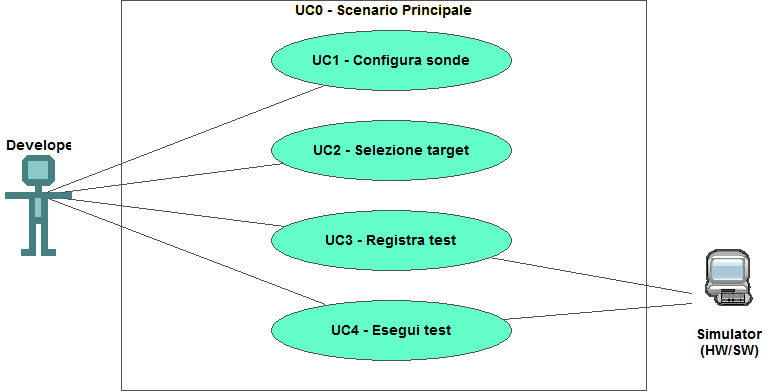
\includegraphics[width=0.9\columnwidth]{usecase/scenario-principale} 
    \caption{Use Case - UC0: Scenario principale}
\end{figure}

\begin{usecase}{0}{Scenario principale}
\usecaseactors{Sviluppatore applicativi}
\usecasepre{Lo sviluppatore è entrato nel plug-in di simulazione all'interno dell'IDE}
\usecasedesc{La finestra di simulazione mette a disposizione i comandi per configurare, registrare o eseguire un test}
\usecasepost{Il sistema è pronto per permettere una nuova interazione}
\label{uc:scenario-principale}
\end{usecase}

\section{Tracciamento dei requisiti}

Da un'attenta analisi dei requisiti e degli use case effettuata sul progetto è stata stilata la tabella che traccia i requisiti in rapporto agli use case.\\
Sono stati individuati diversi tipi di requisiti e si è quindi fatto utilizzo di un codice identificativo per distinguerli.\\
Il codice dei requisiti è così strutturato R(F/Q/V)(N/D/O) dove:
\begin{enumerate}
	\item[R =] requisito
    \item[F =] funzionale
    \item[Q =] qualitativo
    \item[V =] di vincolo
    \item[N =] obbligatorio (necessario)
    \item[D =] desiderabile
    \item[Z =] opzionale
\end{enumerate}
Nelle tabelle \ref{tab:requisiti-funzionali}, \ref{tab:requisiti-qualitativi} e \ref{tab:requisiti-vincolo} sono riassunti i requisiti e il loro tracciamento con gli use case delineati in fase di analisi.

\newpage

\begin{table}%
\caption{Tabella del tracciamento dei requisti funzionali}
\label{tab:requisiti-funzionali}
\begin{tabularx}{\textwidth}{lXl}
\hline\hline
\textbf{Requisito} & \textbf{Descrizione} & \textbf{Use Case}\\
\hline
RFN-1     & L'interfaccia permette di configurare il tipo di sonde del test & UC1 \\
\hline
\end{tabularx}
\end{table}%

\begin{table}%
\caption{Tabella del tracciamento dei requisiti qualitativi}
\label{tab:requisiti-qualitativi}
\begin{tabularx}{\textwidth}{lXl}
\hline\hline
\textbf{Requisito} & \textbf{Descrizione} & \textbf{Use Case}\\
\hline
RQD-1    & Le prestazioni del simulatore hardware deve garantire la giusta esecuzione dei test e non la generazione di falsi negativi & - \\
\hline
\end{tabularx}
\end{table}%

\begin{table}%
\caption{Tabella del tracciamento dei requisiti di vincolo}
\label{tab:requisiti-vincolo}
\begin{tabularx}{\textwidth}{lXl}
\hline\hline
\textbf{Requisito} & \textbf{Descrizione} & \textbf{Use Case}\\
\hline
RVO-1    & La libreria per l'esecuzione dei test automatici deve essere riutilizzabile & - \\
\hline
\end{tabularx}
\end{table}%

    \chapter{Progettazione e codifica}
\label{cap:progettazione-codifica}

\intro{Breve introduzione al capitolo}\\

\section{Tecnologie e strumenti}
\label{sec:tecnologie-strumenti}

Di seguito viene data una panoramica delle tecnologie e strumenti utilizzati.

\subsection*{Tecnologia 1}
Descrizione Tecnologia 1.

\subsection*{Tecnologia 2}
Descrizione Tecnologia 2

\section{Ciclo di vita del software}
\label{sec:ciclo-vita-software}

\section{Progettazione}
\label{sec:progettazione}

\subsubsection{Namespace 1} %**************************
Descrizione namespace 1.

\begin{namespacedesc}
    \classdesc{Classe 1}{Descrizione classe 1}
    \classdesc{Classe 2}{Descrizione classe 2}
\end{namespacedesc}


\section{Design Pattern utilizzati}

\section{Codifica}

    \chapter{Verifica e validazione}
\label{cap:verifica-validazione}

    \chapter{Conclusioni}
\label{cap:conclusioni}

\section{Consuntivo finale}

\section{Raggiungimento degli obiettivi}

\section{Conoscenze acquisite}

\section{Valutazione personale}


    \appendix
    \chapter{Appendix A}
\section{Java vs Python for API Development}
\label{sec:java-vs-python}

In the realm of API development, Java and Python are two of the most used programming languages, each offering distinct features, benefits, and trade-offs. This section will explore these languages, focusing on their usage in API development with Spring Boot for Java and FastAPI for Python.
A study of the pros and cons of each language and framework will help in determining which one is better suited for API development. Besides the personal experience, the information reported here is based on general industry trends and best practices.

\subsection{Java and Spring Boot}

Java is a statically-typed, object-oriented programming language that has been a staple in enterprise-level applications for decades. Its robustness, extensive libraries, and strong community support make it a reliable choice for large-scale systems.

\textbf{Spring Boot} is a framework designed to simplify the development of Java applications. It is part of the larger Spring Framework ecosystem and is widely used for building production-ready standalone applications with minimal configuration.

\textbf{Pros of Java and Spring Boot:}
\begin{itemize}
    \item \textbf{Performance}: Java's statically-typed nature and JVM optimization result in high performance and efficient memory management, which is crucial for large-scale applications.
    \item \textbf{Scalability}: Java applications, particularly those built with Spring Boot, are known for their scalability. Spring Boot's support for microservices architecture allows for easy scaling and maintenance.
    \item \textbf{Security}: Java offers robust security features, and Spring Boot provides built-in security mechanisms, making it easier to develop secure APIs.
    \item \textbf{Mature Ecosystem}: Java has a mature ecosystem with a variety of libraries, tools, and frameworks. Spring Boot, in particular, integrates seamlessly with other Spring projects and third-party tools.
    \item \textbf{Community Support}: Java's long-standing presence in the industry means it has extensive community support and documentation, which can be invaluable for troubleshooting and development.
\end{itemize}

\textbf{Cons of Java and Spring Boot:}
\begin{itemize}
    \item \textbf{Complexity}: Java's syntax and the Spring Boot framework can be complex and verbose, leading to a steeper learning curve for beginners.
    \item \textbf{Configuration}: Although Spring Boot reduces the configuration overhead compared to traditional Spring applications, it can still be more cumbersome compared to the lightweight configurations in some other languages. A non-experienced developer may find it challenging to set up.
\end{itemize}

\subsection{Python and FastAPI}

Python is a dynamically-typed, interpreted language known for its simplicity and readability. Its versatility and ease of use have made it popular across various domains, including web development, data science, and automation.

\textbf{FastAPI} is a modern, high-performance web framework for building APIs with Python 3.7+ based on standard Python type hints. It is designed to be easy to use and offers automatic interactive API documentation.

\textbf{Pros of Python and FastAPI:}
\begin{itemize}
    \item \textbf{Ease of Use}: Python's simple and readable syntax makes it accessible to beginners and allows for rapid development.
    \item \textbf{Fast Development}: FastAPI leverages Python's dynamic capabilities and type hints to provide features like automatic data validation and interactive API documentation, accelerating development.
    \item \textbf{Flexibility}: Python is highly flexible, and FastAPI's design allows developers to easily integrate with other libraries and tools.
    \item \textbf{Asynchronous Support}: FastAPI natively supports asynchronous programming, making it well-suited for applications requiring high concurrency.
    \item \textbf{Automatic Documentation}: FastAPI automatically generates interactive API documentation using Swagger UI and ReDoc, which is highly beneficial for development and testing.
\end{itemize}

\textbf{Cons of Python and FastAPI:}
\begin{itemize}
    \item \textbf{Performance}: Python, being an interpreted language, is generally slower than compiled languages like Java. This can be a drawback for CPU-intensive tasks.
    \item \textbf{Scalability}: While Python applications can be scaled, it often requires more effort and optimization compared to Java applications. FastAPI, however, improves this aspect with its asynchronous capabilities.
    \item \textbf{Type Safety}: Python's dynamic typing can lead to runtime errors that are not caught at compile time, which can affect the reliability of the code.
\end{itemize}

\subsection{Why Java is a Better Option}

When comparing Java with Spring Boot and Python with FastAPI for API development, Java tends to be a better option for several reasons:

\begin{itemize}
    \item \textbf{Performance and Efficiency}: Java's performance, aided by the JVM, is superior to Python. For API development, where high throughput and low latency are critical, Java's efficiency makes a significant difference.
    \item \textbf{Enterprise-Grade Scalability}: Java's robust ecosystem and the comprehensive features of Spring Boot make it well-suited for large-scale, enterprise-level applications. The scalability and maintainability of Java applications are generally higher, making them ideal for businesses expecting substantial growth.
    \item \textbf{Security}: Java's strong type system and Spring Boot's extensive security features provide a solid foundation for developing secure APIs. This is particularly important for applications handling sensitive data.
    \item \textbf{Community and Ecosystem}: The extensive community support and the mature ecosystem of libraries and frameworks in Java are crucial advantages. Developers have access to a variety of resources, making it easier to find solutions to problems and ensuring long-term project viability.
    \item \textbf{Stability and Reliability}: Java's long history in enterprise environments has proven its stability and reliability. Businesses often prefer Java for critical applications due to its consistent performance and predictable behavior.
\end{itemize}

While Python with FastAPI offers ease of use and rapid development, especially for smaller projects or prototyping, Java with Spring Boot stands out as a more robust, scalable, and secure choice for developing APIs, especially in large-scale and performance-intensive enterprise-level scenarios.







    \backmatter
    \printglossary[type=\acronymtype, title=Acronimi e abbreviazioni, toctitle=Acronimi e abbreviazioni]
    \printglossary[type=main, title=Glossario, toctitle=Glossario]

    \cleardoublepage
\chapter{Bibliografia}

\nocite{*}

% Print book bibliography
\printbibliography[heading=subbibliography,title={Riferimenti bibliografici},type=book]

% Print site bibliography
\printbibliography[heading=subbibliography,title={Siti web consultati},type=online]

\end{document}
